\documentclass[dvisvgm,tikz,margin=2pt]{standalone}
\usepackage{amsmath,amssymb,amsthm}
\usepackage{tikz}
\usetikzlibrary{patterns}
\usepackage{xcolor}
\newcommand{\R}{\mathbb{R}}
\newcommand{\vol}{\operatorname{vol}}
\newcommand{\HV}{\operatorname{HV}}
\newcommand{\Oh}{\mathcal{O}}
\begin{document}
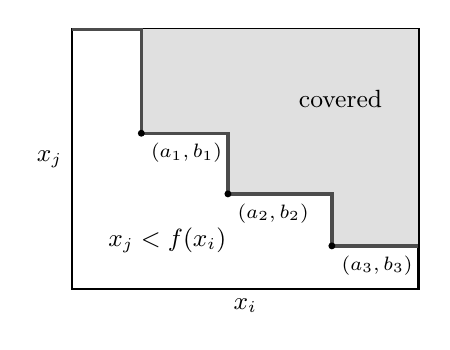
\begin{tikzpicture}[scale=2.2]
  \draw[thick] (0,0) rectangle (2,1.5);
  \fill[black!12] (0.4,0.9) rectangle (2,1.5);
  \fill[black!12] (0.9,0.55) rectangle (2,1.5);
  \fill[black!12] (1.5,0.25) rectangle (2,1.5);
  \draw[very thick] (0,1.5);
  \draw[very thick,black!70]
    (0,1.5) -- (0.4,1.5) -- (0.4,0.9) -- (0.9,0.9) -- (0.9,0.55)
    -- (1.5,0.55) -- (1.5,0.25) -- (2,0.25);
  \fill (0.4,0.9) circle (0.02) node[below right] {\scriptsize $(a_1,b_1)$};
  \fill (0.9,0.55) circle (0.02) node[below right] {\scriptsize $(a_2,b_2)$};
  \fill (1.5,0.25) circle (0.02) node[below right] {\scriptsize $(a_3,b_3)$};
  \node at (1.55,1.1) {\small covered};
  \node at (0.55,0.28) {\small $x_j<f(x_i)$};
  \node[below] at (1,0) {\small $x_i$};
  \node[left] at (0,0.75) {\small $x_j$};
\end{tikzpicture}
\end{document}
